% This tex file is available under a
% Creative Commons Attribution-Share Alike license (CC BY-SA 2.0).
% http://creativecommons.org/licenses/by-sa/2.0/
% Copyright © 2013 Rodrigo Hausen
\documentclass{beamer}
\usepackage[utf8]{inputenc}
\usepackage{lmodern}
\usepackage[T1]{fontenc}
\usepackage[portuguese,brazil]{babel}
\usepackage{url}
\usepackage{listings}
\usepackage{color}
\usepackage{textcomp}
\usepackage{pdfpages}
\usepackage{fancyvrb}
\usepackage{enumerate}
\usepackage{alltt}
\usepackage{array}
\usepackage{slashbox}
%\usepackage[pdf]{pstricks}
%\usepackage{auto-pst-pdf}
%\usepackage{icomma} % para vírgula decimal / decimal comma
\definecolor{listinggray}{gray}{0.9}
\definecolor{mediumgray}{rgb}{0.6,0.6,0.6}
\definecolor{lbcolor}{rgb}{0.9,0.9,0.9}
\lstset{
    backgroundcolor=\color{lbcolor},
    tabsize=4,
    rulecolor=,
    basicstyle=\scriptsize,
    upquote=true,
    aboveskip={1.5\baselineskip},
    columns=fixed,
    showstringspaces=false,
    extendedchars=true,
    breaklines=true,
    prebreak = \raisebox{0ex}[0ex][0ex]{\ensuremath{\hookleftarrow}},
    frame=single,
    showtabs=false,
    showspaces=false,
    showstringspaces=false,
    identifierstyle=\ttfamily,
    keywordstyle=\color[rgb]{0,0,1},
    commentstyle=\color[rgb]{0.133,0.545,0.133},
    stringstyle=\color[rgb]{0.627,0.126,0.941},
}
\definecolor{pinegreen}{RGB}{0,139,114}
\definecolor{pgr}{RGB}{0,139,114}

\definecolor{aquamarine}{RGB}{0,181,190}
\definecolor{aqm}{RGB}{0,181,190}

\definecolor{skyblue}{RGB}{100,227,251}
\definecolor{skb}{RGB}{100,227,251}

\definecolor{pnk}{RGB}{255,150,150}

\newcommand{\comment}[1]{{\color{structure.fg!70!white}\footnotesize #1}}

\newcommand{\WD}[1]{\fbox{#1}\hspace{-0.5pt}}
\newcommand{\FWD}[1]{%
\fbox{%
\vbox to 10pt{\vfil%
\hbox to 0.8cm{\hfill#1\hfill}%
\vfil}%
}\hspace{-0.5pt}%
}

\def\A{\texttt{A}}
\def\B{\texttt{B}}
\def\C{\texttt{C}}
\def\D{\texttt{D}}
\def\E{\texttt{E}}
\def\F{\texttt{F}}

\usetheme{Boadilla}
%\usetheme{umbc2}
\usefonttheme{structuresmallcapsserif}
\usecolortheme{seahorse}

\title{Aula 12: Circuitos Digitais Sequenciais -- Latches}
\subtitle{Circuitos Digitais}
\author{Rodrigo Hausen}
\institute{CMCC -- UFABC} 
\date{8 de março de 2013}

\newcommand{\Not}[1]{\overline{#1}}
\def\And{\,}

\begin{document}

\begin{frame}
\maketitle

\vspace{-1cm}

\begin{center}
\url{http://compscinet.org/circuitos}
\end{center}

\end{frame}

%%%%%%%%%%%%%%%%%%%%%%%%%%%%%%%%%%%%%%%%%%%%%%%%%
\begin{frame}
\frametitle{Circuitos Digitais Combinacionais}

\begin{itemize}
\item Até agora, todos os circuitos digitais que estudamos
      possuem uma propriedade em comum:\\
      O estado das saídas depende \textbf{única e exclusivamente}
      do estado \textbf{atual} das entradas.
\pause
\item Tais circuitos são classificados como \textbf{circuitos digitais
      combinacionais}.
	\begin{itemize}
	\item circuitos combinacionais não guardam nenhuma informação
              sobre estados anteriores (ausência de memória)
	\end{itemize}
\pause
\item Alguns circuitos digitais, ao contrário, podem guardar informação
      sobre estados anteriores. Tais circuitos são chamados de
      \textbf{circuitos digitais sequenciais}.
	\begin{itemize}
	\item em circuitos sequenciais, o estado das saídas depende não
              apenas do estado atual das entradas, \textbf{mas também de
              estados anteriores das entradas e/ou saídas} (presença de
              memória).
	\end{itemize}
\end{itemize}
\end{frame}

%%%%%%%%%%%%%%%%%%%%%%%%%%%%%%%%%%%%%%%%%%%%%%%%%
\begin{frame}
\frametitle{Circuitos Digitais Sequenciais}
\begin{itemize}
\item Exemplo de um circuito digital sequencial:\\[6pt]
      \begin{center}
        
\includegraphics{images/circuit1}
      \end{center}
\pause
\item A tabela verdade de um circuito digital sequencial depende
      de estados anteriores.
\pause
\item Usaremos $X_i$ para denotar o estado \textbf{atual} da saída e
$X_{i-1}$ para denotar o estado anterior.
\pause
\begin{center}
\begin{tabular}{cc||c}
$A$ & $X_{i-1}$ & $X_i$ \\
\hline
 0  &     0     &   0   \\ \pause
 1  &     0     &   1   \\ \pause
 0  &     1     &   1   \\ \pause
 1  &     1     &   1
\end{tabular}
\end{center}
\pause
\item Outra notação (Floyd): estado atual = $X$, estado anterior = $X_0$
\end{itemize}

\end{frame}

%%%%%%%%%%%%%%%%%%%%%%%%%%%%%%%%%%%%%%%%%%%%%%%%%
\begin{frame}
\frametitle{Circuitos Digitais Sequenciais}

Esboce o diagrama de forma de onda para a saída $X$, considerando
o diagrama de forma de onda para a entrada $A$, e que até o instante
$t_1$ o estado de $X$ é $0$.

\begin{center}
	
\includegraphics{images/circuit1}
\end{center}

\vspace{-24pt}

\begin{center}
\only<1,3>{\includegraphics[scale=0.9]{images/wave1_4}}%
\only<2>{\includegraphics[scale=0.9]{images/wave1_5}}
\only<4>{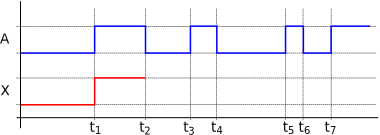
\includegraphics[scale=0.9]{images/wave1_3}}%
\only<5>{\includegraphics[scale=0.9]{images/wave1_2}}%
\only<6>{\includegraphics[scale=0.9]{images/wave1_1}}%
\only<7->{\includegraphics[scale=0.9]{images/wave1_0}}%
\end{center}

\vspace{-10pt}

\uncover<8->{O circuito identifica se em algum instante a
entrada passou para nível alto.}
\end{frame}

%%%%%%%%%%%%%%%%%%%%%%%%%%%%%%%%%%%%%%%%%%%%%%%%%
\begin{frame}
\frametitle{Circuitos Digitais Sequenciais}

Outro exemplo: construa a tabela verdade e esboce o diagrama de
forma de onda para a saída $X$ abaixo, considerando que o estado
inicial de $A$ é $0$ e de $X$ é $1$.

\vspace*{\fill}

\begin{center}
	\includegraphics{images/circuit2}
\end{center}

\vspace*{\fill}

(Solução na lousa)

\end{frame}

%%%%%%%%%%%%%%%%%%%%%%%%%%%%%%%%%%%%%%%%%%%%%%%%%
\begin{frame}
\frametitle{Feedback}

\begin{itemize}
\item Característica comum aos circuitos digitais sequenciais:\\
presença de \emph{feedback} (realimentação)
\end{itemize}

\hspace*{\fill}%
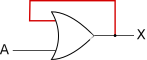
\includegraphics{images/circuit1_feed}%
\hspace*{\fill}%
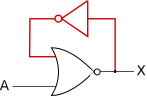
\includegraphics{images/circuit2_feed}%
\hspace*{\fill}
\end{frame}

%%%%%%%%%%%%%%%%%%%%%%%%%%%%%%%%%%%%%%%%%%%%%%%%%
\begin{frame}
\frametitle{Latch do tipo $R$-$S$ (Reset-Set)}

\begin{itemize}
\item Faça a tabela verdade do circuito abaixo e esboce o diagrama
      de forma de onda para as saídas $Q$ e $P$, considerando a seguinte
      sequência de estados para as entradas:
	\begin{enumerate}
	\item $R = 1, S = 0$;
	\item $R = 0, S = 0$;
	\item $R = 0, S = 1$;
	\item $R = 0, S = 0$.
	\end{enumerate}
      Desconsidere, por enquanto, o estado $R = 1, S = 1$.
\end{itemize}
\begin{center}
\includegraphics{images/circuit3}
\end{center}

\end{frame}

%%%%%%%%%%%%%%%%%%%%%%%%%%%%%%%%%%%%%%%%%%%%%%%%%
\begin{frame}
\frametitle{Latch do tipo $R$-$S$ (Reset-Set)}

\begin{itemize}
\item A saída $P$ é sempre o inverso de $Q$.\\
      Passaremos a chamar a saída $P$ de $\Not{Q}$.
\pause
\item A tabela verdade desse circuito pode ser escrita como:
\begin{tabular}{cc||ccl}
$R$ & $S$ & $Q_i$ & $\Not{Q_i}$ \\
\cline{1-4}
 1  &  0  &   0   &     1       & (reset $Q$) \\ \pause
 0  &  1  &   1   &     0       & (set $Q$) \\ \pause
 0  &  0  & $Q_{i-1}$ & $\Not{Q_{i-1}}$ & (mantém $Q$) \pause
\end{tabular}
\pause
\item Este circuito é chamado \textbf{\emph{latch} R-S}\\[6pt]
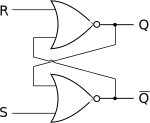
\includegraphics[scale=0.85]{images/latchRS_circuit}\pause
\hspace{6ex}
\raisebox{40pt}{\Huge$=$}
\hspace{6ex}\pause
\includegraphics[scale=0.85]{images/latchRS_blackbox}
\end{itemize}

\end{frame}

%%%%%%%%%%%%%%%%%%%%%%%%%%%%%%%%%%%%%%%%%%%%%%%%%
\begin{frame}
\frametitle{Latch do tipo $R$-$S$ (Reset-Set)}

\begin{itemize}
\item E o estado $R = 1, S = 1$?
\pause
\item Esboce os diagramas de forma de onda para $Q$ e $\Not{Q}$,
      considerando $R$ e $S$ conforme o diagrama abaixo.
\begin{center}
\only<1-2>{\includegraphics[scale=0.9]{images/waveformRS_6}}%
\only<3>{\includegraphics[scale=0.9]{images/waveformRS_5}}%
\only<4>{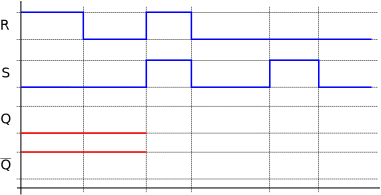
\includegraphics[scale=0.9]{images/waveformRS_4}}%
\only<5>{\includegraphics[scale=0.9]{images/waveformRS_2}}%
\only<6>{\includegraphics[scale=0.9]{images/waveformRS_1}}%
\only<7>{\includegraphics[scale=0.9]{images/waveformRS_0}}%
\only<8->{\includegraphics[scale=0.9]{images/waveformRS}}%
\end{center}
\pause\pause\pause\pause\pause\pause\pause
\item Após a uma transição $R=1,S=1$ para $R=0,S=0$ as saídas
ficam instáveis, só voltando ao normal após o próximo reset ou set.
\end{itemize}
\end{frame}

%%%%%%%%%%%%%%%%%%%%%%%%%%%%%%%%%%%%%%%%%%%%%%%%%
\begin{frame}
\frametitle{Latch do tipo $R$-$S$ (Reset-Set)}

\centering
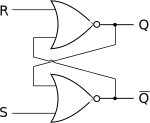
\includegraphics{images/latchRS_circuit}
\hspace{6ex}
\raisebox{40pt}{\Huge$=$}
\hspace{6ex}
\includegraphics{images/latchRS_blackbox}\\

\vspace{12pt}

\begin{center}
\begin{tabular}{cc||ccl}
$R$ & $S$ & $Q_i$ & $\Not{Q_i}$ \\
\cline{1-4}
 1  &  0  &   0   &     1       & (reset $Q$) \\
 0  &  1  &   1   &     0       & (set $Q$) \\
 0  &  0  & $Q_{i-1}$ & $\Not{Q_{i-1}}$ & (mantém $Q$) \\
 1  &  1  &   X   &     X       & (estado proibido)
\end{tabular}
\end{center}
\end{frame}

%%%%%%%%%%%%%%%%%%%%%%%%%%%%%%%%%%%%%%%%%%%%%%%%%
\begin{frame}
\frametitle{Latch do tipo $\Not{S}$-$\Not{R}$ com portas NAND}

\begin{itemize}
\item É possível construir um latch similar com portas NAND, mas as
entradas se tornam \textbf{ativas em nível baixo}.
\end{itemize}

\pause

\begin{center}
\includegraphics{images/latchRSnand_circuit}\pause
\hspace{6ex}
\raisebox{40pt}{\Huge$=$}\pause
\hspace{6ex}
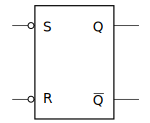
\includegraphics{images/latchRSnand_blackbox}\\

\vspace{12pt} \pause

\begin{tabular}{cc||ccl}
$\Not{S}$ & $\Not{R}$ & $Q_i$ & $\Not{Q_i}$ \\
\cline{1-4}
 1  &  0  &   0   &     1       & (reset $Q$) \\
 0  &  1  &   1   &     0       & (set $Q$) \\
 1  &  1  & $Q_{i-1}$ & $\Not{Q_{i-1}}$ & (mantém $Q$) \\
 0  &  0  &   X   &     X       & (estado proibido)
\end{tabular}
\end{center}
\end{frame}

%%%%%%%%%%%%%%%%%%%%%%%%%%%%%%%%%%%%%%%%%%%%%%%%%
\begin{frame}
\frametitle{Circuito de habilitação (enable)}

\begin{itemize}
\item \textbf{Problema 1}: considere o circuito abaixo. Qual é o estado
de cada saída $X$ e $Y$ quando $En = 0$ e quando $En = 1$?

\vspace{12pt}

\begin{center}
\only<1,4->{\includegraphics{images/enable_circuit}}%
\only<2>{\includegraphics{images/enable_circuit0}}%
\only<3>{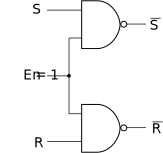
\includegraphics{images/enable_circuit1}}%
%
\hspace{6ex}%
%
\uncover<4->{
\raisebox{60pt}{
\begin{tabular}{c||cc}
$En$ & $X$ & $Y$ \\
\hline
  0  &  1  &  1  \\
  1  & $\Not{S}$ & $\Not{R}$
\end{tabular}
}
}
\end{center}
\end{itemize}

\end{frame}

%%%%%%%%%%%%%%%%%%%%%%%%%%%%%%%%%%%%%%%%%%%%%%%%%
\begin{frame}
\frametitle{Circuito de habilitação (enable)}

\begin{itemize}
\item Circuito de habilitação com portas NAND torna as entradas $S$ e $R$:
\begin{itemize}
\item Se $En = 1$: ativas em nível baixo, ou seja, $\Not{S}$ e $\Not{R}$;
\item Se $En = 0$, desabilitadas
\end{itemize}
\end{itemize}

\begin{center}
\includegraphics{images/enable_circuit}
\end{center}

\pause

\begin{itemize}
\item a entrada $En$ é chamada \textbf{entrada de habilitação} (enable input)
\end{itemize}

\end{frame}

%%%%%%%%%%%%%%%%%%%%%%%%%%%%%%%%%%%%%%%%%%%%%%%%%
\begin{frame}
\frametitle{Latch do tipo $S$-$R$ com enable}

\begin{center}
\only<1>{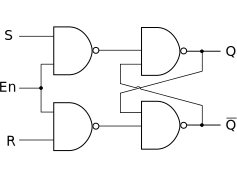
\includegraphics{images/latchRSnandEnable_circuit}}%
\only<2,5->{\includegraphics{images/latchRSnandEnable_circuit1}}%
\only<3>{\includegraphics{images/latchRSnandEnable_circuit_enabled}}%
\only<4>{\includegraphics{images/latchRSnandEnable_circuit_disabled}}%
\uncover<6->{%
\raisebox{68pt}{\Huge=}%
}%
\uncover<7->{%
\raisebox{24pt}{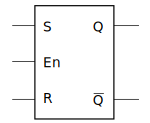
\includegraphics{images/latchRSenable_blackbox}}%
}

\vspace{6pt}

\uncover<8->{
\begin{tabular}{ccc||cl}
$En$ & $S$ & $R$ & $Q_i$ \\
\cline{1-4}
 1   &  0  &  1  &   0  & (reseta $Q$) \\
 1   &  1  &  0  &   1  & (seta $Q$) \\
 1   &  0  &  0  & $Q_{i-1}$  & (mantém $Q$) \\
 0   &  ?  &  ?  & $Q_{i-1}$  & (mantém $Q$, não importa $R$ nem $S$) \\
\end{tabular}
}
\end{center}
\end{frame}

%%%%%%%%%%%%%%%%%%%%%%%%%%%%%%%%%%%%%%%%%%%%%%%%%
\begin{frame}
\frametitle{Latch do tipo $D$ (data)}

\begin{itemize}
\item A inclusão da entrada $En$ é uma conveniência a mais no latch $S$-$R$,
      e permite uma outra forma de manter o estado do latch.
\pause
\item Porém, ainda temos que nos preocupar em nunca fazer $S = 1$ e $R = 1$
      enquanto o latch estiver habilitado ($En = 1$).
\pause
\item O uso de uma única entrada para set/reset evita esse problema:\\[12pt]
\begin{center}
\includegraphics{images/latchD}
\end{center}
\end{itemize}
\end{frame}

%%%%%%%%%%%%%%%%%%%%%%%%%%%%%%%%%%%%%%%%%%%%%%%%%
\begin{frame}
\frametitle{Latch do tipo $D$ (data)}

\hspace*{\fill}
\includegraphics{images/latchD}%
\hspace*{\fill}\pause%
\raisebox{40pt}{\Huge=}%
\hspace*{\fill}\pause%
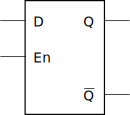
\includegraphics{images/latchD_blackbox}%
\hspace*{\fill}

\vspace{12pt}

\pause

\begin{center}
\begin{tabular}{cc||cl}
$D$ & $En$ & $Q_i$  \\
\cline{1-3}
 0  &   1  &   0   & (reset) \\
 1  &   1  &   1   & (set) \\
 ?  &   0  & $Q_{i-1}$ & (mantém, sem se importar com $D$) \\
\end{tabular}
\end{center}

\end{frame}

%%%%%%%%%%%%%%%%%%%%%%%%%%%%%%%%%%%%%%%%%%%%%%%%%
\begin{frame}
\frametitle{Latch $D$: aplicação}

Registrador de armazenamento: armazena uma palavra de dado\\[6pt]

\begin{center}
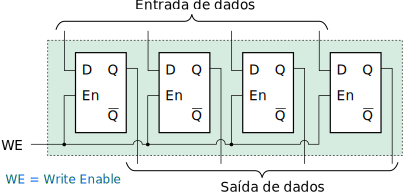
\includegraphics[scale=0.8]{images/register}\pause\\[6pt]
\raisebox{24pt}{\Huge=}\hspace{6ex}\pause
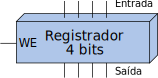
\includegraphics{images/register_blackbox}\\
\end{center}

\end{frame}

%%%%%%%%%%%%%%%%%%%%%%%%%%%%%%%%%%%%%%%%%%%%%%%%%
\begin{frame}
\frametitle{Para Casa}

\begin{itemize}
\item Ler seção 7-1
\item Exercícios: autoteste 1--3, problemas 1--7
\end{itemize}
\pause
\textbf{Exercício adicional:} usando decodificadores, multiplexadores e registradores, projete uma memória para 16 palavras de $4$ bits cada:
\begin{itemize}
\item $4$ saídas de dados: $D_3, D_2, D_1, D_0$
\item $4$ entradas de dados: $d_3, d_2, d_1, d_0$
\item $4$ entradas de endereço: $a_3, a_2, a_1, a_0$
\item $1$ entrada de operação: $Op$ 
\pause
\item Se $Op = 0$, a palavra de dados contida
          no registrador de número $(a_3, a_2, a_1, a_0)_2$ será
          colocada nas saídas de dados
\pause
\item Se $Op = 1$, a palavra de dados nas entradas de dados será
          gravada no registrador de número $(a_3, a_2, a_1, a_0)_2$
\pause
\item Para facilitar, use notação de barramento
\end{itemize}
\end{frame}

\end{document}
